% Capítulo 6
\chapter{Estudo Experimental}
\label{cap:cap6}

este capítulo consiste em apresentar o estudo por meio de método experimental, envolve a concepção do contexto do experimento, da disposição e características dos elementos envolvidos, a seleção das variáveis influenciadoras, o controle e a instrumentação do experimento, sua execução, a captura de dados durante experimentação, e por fim, a análise e conclusões obtidas a partir desses resultados. 

O objetivo do experimento é analisar a viabilidade do uso de mecanismos de \textit{throttling} já apresentados como candidato para aumentar a disponibilidade dos elementos presentes em \textit{IoT} através do ajuste de comportamento por ação de limiares de atuação que consideram seus aspectos energéticos e com isso prolongar a autonomia energética dos dispositivos. A abordagem é aderente aos elementos presentes na taxonomia proposta no Capítulo \ref{cap:cap4} e permite comparação e análise entre dispositivos que diferem sobre o fato de terem sua operação ajustada mediante \textit{throttling} ou não. 

\begin{figure}[H]
	\centering
	\caption{Etapas do Estudo Experimental.}
	\label{fig:cap6metodologia}
	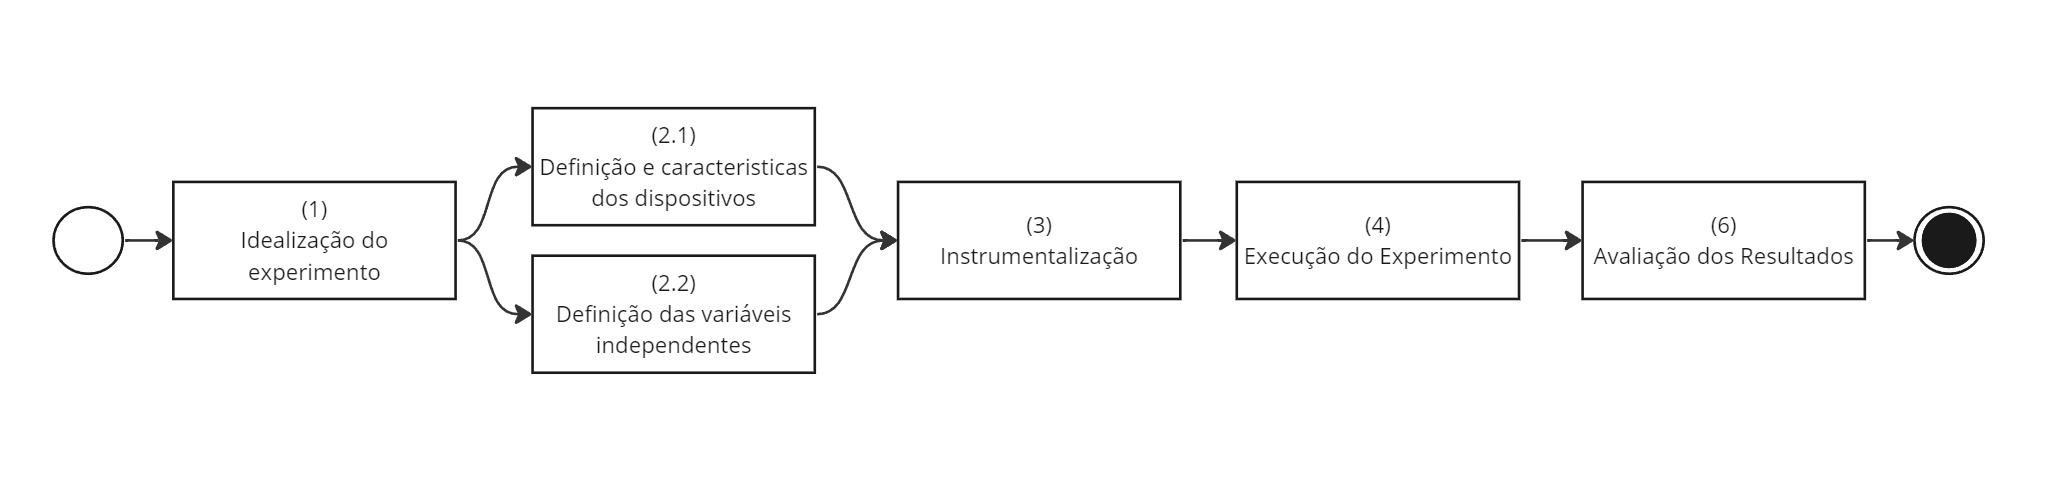
\includegraphics[width=1\linewidth]{Imagens/cap6/cap6metodologia.jpg}
	
	Fonte: elaborado pelo autor.
\end{figure} 


\section{Metodologia}

O experimento pretende comparar os efeitos do mecanismo de \textit{throttling} em dispositivos com capacidade de coleta de energia, com foco em examinar a disponibilidade de cada um relacionada aos aspectos energéticos em condições de capacidade e atuação semelhantes.

Para tal, buscou-se observar a influência do fator limitante na alteração do comportamento dos participantes em relação aos valores de energia coletada e reserva energética. Além disso, buscou-se compreender sua eficiência na tomada de decisão em atender ou não às solicitações, em virtude da autoanálise de suas capacidades à medida que a variação de energia disponível ocorre. Este estudo visa analisar o uso de \textit{throttling} como possível solução para estender a disponibilidade de dispositivos com capacidade de coleta energética. 

Na Etapa 1 idealização do experimento, foi concebido quais os temos de projeto para viabilizar a análise e comparação do padrão em detrimento dos objetivos propostos.  A Figura \ref{fig:cap6metodologia} apresenta o fluxo das etapas realizadas no processo. Inicialment, foi projetado ambiente para abstrair os elementos envolvidos, visando garantir equidade de condições e ações de maneira simultânea para todos os dispositivos durante a simulação. Para alcançar isolamento e consistência, optou-se pelo uso da plataforma Docker\footnote{O Docker é uma plataforma de virtualização que simplifica o desenvolvimento, envio e execução de aplicativos em contêineres. Disponível em \url{https://www.docker.com/}.} como agente facilitador, que atende às restrições necessárias de encapsulamento para que cada aplicação e suas dependências estejam contidas. 

Conforme ilustrado na Figura <DIAGRAMA DE BLOCO DO SISTEMA>, essa abordagem permite que ambos os sistemas fossem estimulados paralelamente, mantendo controle sobre seus recursos e garantindo os termos de operação (capacidade de processador, memória e disco). Sendo assim, a composição do experimento considera que:  I - Dispositivos com capacidade de coleta e armazenamento de energia estão inseridos em um dado ambiente de simulação controlada; II - Os dispositivos sempre recebem simultaneamente o mesmo valor como coleta de energia; III - Os dispositivos participantes possuem a mesma capacidade de armazenamento para energia coletada; IV - Os dispositivos são submetidos simultaneamente a mesma quantidade de solicitações, os ciclos de carga.

Na Etapa 3, abordado-se o processo de instrumentalização do ambiente simulado, essencial meio para apresentar os resultados durante a execução do experimento e posterior resumo dos dados obtidos, seus detalhes estão descritos na Seção \ref{SECAO INSTRUMENTACAO}. A Seção \ref{SECAO EXECUCAO} descreve os processos de execução do experimento Etapa 4, aqui todas as etapas planejadas anteriormente ja estão implementadas. Sendo assim, os procedimentos são realizados conforme o protocolo estabelecido, e aplicação dos estímulos definidos  (carga de solicitações e disponibilização de recursos na forma de coleta energética). Durante esta fase, a precisão e a consistência são fundamentais para garantir a validade dos resultados analisados na próxima fase. 

Ao final, a Etapa 5 trata dos dados coletados para análise e avaliação,
consistindo em: I - Medição dos valores energéticos em relação ao tempo; II - Quantidade de solicitações atendidas ou negadas; III - Valores mínimos de reserva energética atingidos. Tais resultados serão melhores descritos posteriormente e apresentam o escopo de comparação entre os elementos participantes fundamento em que se baseia a avaliação dos resultados descritos na Seção \ref{SECAO AVALIACAO RESULTADOS}.

\section{Idealização}
O cenário experimentado simula a atuação de nodes em dado ambiente externo. Estes nodes são concebidos com capacidade de coletar energia no meio onde estão inseridos, esta é considerada entrada energética para o funcionamento do node. Também é possível armazenar parte do recurso energético coletado e, por fim, a capacidade de resposta com a aferição de um dado simbólico qualquer do meio quando solicitado. Este node é considerado provedor, a medida que atende solicitações de tais aferições.

\section{Definição dos dispositivos e variáveis independentes.}
\section{Instrumentalização.}
\section{Execução.}
\section{Avaliação.}
 